\section{Methodology}

In this section we will describe the prestudy done before choosing the methodology
in this project. In the end in this section, there will be a conclusion of what we have
chosen and why we did so.

\subsection{Waterfall}

{\bf The waterfall process } is a sequential design process that 'flows' through the phases like a waterfall.
The waterfall process is also known as the 'standard' process because it was the most popular process before
agile processes became popular. 

With the waterfall process there is only one distinct goal for each phase. One can imagine a waterfall on the cliff of a steep mountain. Once the water is flowing over the edge of the cliff, it cannot turn back. The same applies to waterfall development. \cite{wikiWaterfall, techtargetWaterfall}

{\bf The phases of the waterfall model:} There are five main phases in a normal waterfall process. 
Here is a briefly description:
\begin{itemize}
	\item {\bf Requirement specification:} Is the phase where the requirements are collected, functional and non-functional, to make a complete description of the behaviour of the system to be developed.
	\item {\bf Design: } Is the phase where the requirements are used to make the overall design of the system such as the
	architecture.
	\item {\bf Implementation:} Is where the development of the designed system is done. In the implementation phase, 
	it is also common that some kind of testing takes place during implementation.
	\item {\bf Verification (testing and installation): } When the implementation is done, the solution needs to be tested and installed.
	\item {\bf Maintainance:} Is the modification of a software product after delivery to correct errors, to improve performance or other attributes.
\end{itemize}

{\bf Pros: }
\begin{itemize}
	\item Simple and easy to understand and use
	\item Phases are processed and completed one at a time.
	\item Works in projects where the requirements are well understood (low risk of the requirements being changed)
\end{itemize}

{\bf Cons: }
\begin{itemize}
	\item It is very difficult to change the requirement specification, so it is not suitable for the projects where requirements are at a moderate to high risk of changing.
	\item No delivery of working software until the end of the project. This can be critical because the customer may not
	be able to be a part of the process and this may result in an unhappy customer.
\end{itemize}

\begin{figure}[!ht]
\centering
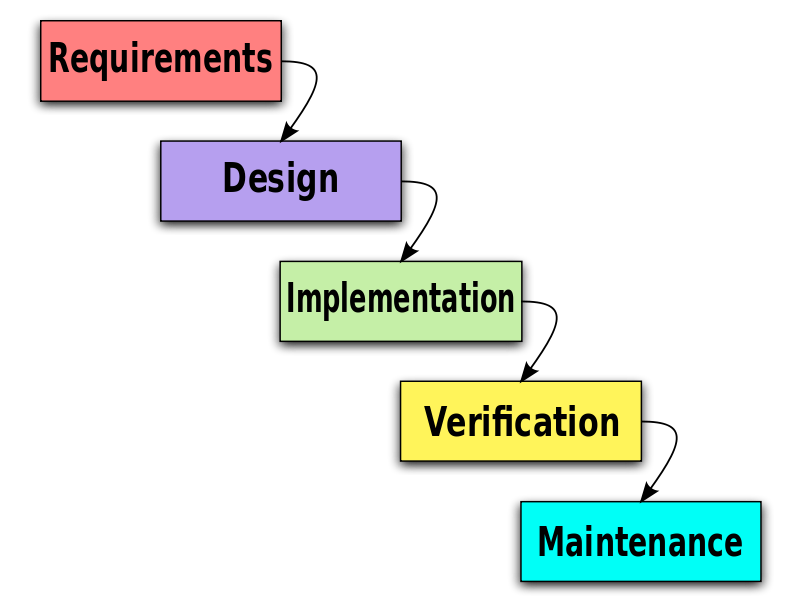
\includegraphics[scale=0.3]{pictures/Waterfall_model.png}
\caption{The waterfall process}
\label{overflow}
\end{figure}


\subsection{Scrum}
{\bf The scrum process: } Scrum is an agile iterative process with focus on small deliveries. The process
defines a self-sustaining team ("The Scrum Team") that defines the goal for each phase. The goal 
is achived through small product increments in iteration that normally last for 1-4 weeks. 
All the functions to implement is planned and is added to a list called a "Product Backlog". The
functions is normally defined as user stories and is added in a prioritized order. In each increment, 
in scrum called a "Sprint", there is a sprint meeting where the scrum team pick userstories from the 
product backlog and add them to the "Sprint Backlog". The sprint backlog is the description of what 
to deliver in the end of the sprint.

Because it is a flat structure there is a concept in scrum called "daily standup". This will keep the team together and everyone will be able to get a quick status update. It usually lasts only 5-15 minutes. 

In a scrum process the stakeholders are a part of the team. The stakeholders will be able to give
feedback in every sprint in terms of changes or approval of a delivery in what is called a "sprint review".
In other methodologies, the stakeholders are only a part of a big delivery in the end, and will 
make it difficult to make changes to what is developed. In scrum, each sprint is a small delivery.

{\bf Pros: }
\begin{itemize}
	\item Small deliveries with feedback from stakeholders
	\item Opportunity to make changes to the requirements during the process
	\item Flat structure (this will adapt to small and bigger teams)
	\item Daily status update from daily standup meetings
	\item Fits for small teams
\end{itemize}

{\bf Cons: }
\begin{itemize}
	\item Require the stakeholders (the customer) to be a part of the team and participate during the process.
\end{itemize}

\subsection{Conclusions}
This section described two different methodologies that were considered as possible methodologies for this project. Because the project is to develop a game with few requirements from the customer, there is a need for a process that will adapt to constant changes in the requirement specification. The waterfall process will not support this and it will be hard to use such process. The scrum process is more likely to fit this project in terms of the amount of planning, 
number of team members and also the high possibility for changes to the requirements.



